\subsection{Ejemplo de implementación en un Sistema de Recomendación de tiempo real}

Como punto de partida a esta sección, se aclara que este trabajo de tesis no cubre la implementación del RS propiamente dicho. No obstante, tal como se plantea en la Sección \ref{sec:objetivo_general}, persigue como objetivos la construcción de una arquitectura Big Data para ser aplicada a un gran volumen de datos reales de entrada de texto, y el desarrollo de un nuevo método sobre esta arquitectura, basado en ensambles de clustering, para implementar la matriz de similaridad de texto asociada al RS para sitios de CQA. Para tal fin, se propone en esta sección un ejemplo de RS en tiempo real, para brindar un contexto de aplicación real del presente trabajo. El ejemplo será desarrollado teniendo en cuenta tres casos de uso diferentes: \begin{enumerate*} [label=(\roman*)] \item un proceso fuera de línea ejecutado periódicamente que actualizará la base de datos, caso de uso central de este trabajo y en el cual se sustenta toda la arquitectura propuesta, y que también puede pensarse como una parte integrante de la implementación propuesta en este apartado; \item el punto de vista del usuario que consulta una pregunta en el sitio; y \item el caso (opcional) en que el usuario agrega una nueva pregunta al sitio.\end{enumerate*}

\bigskip A continuación, entonces, veremos el desarrollo de un ejemplo acerca de cómo funcionarían en la práctica los tres casos de uso más frecuentes de aplicación que incorporan las ideas presentadas en esta Tesis.

\subparagraph{El proceso completo del Sistema de Recomendación}
De acuerdo a lo mencionado en el apartado anterior, la propuesta ejemplo de un Sistema de Recomendación completo se puede analizar teniendo en cuenta tres casos de usos, el primero de los cuales se basa directamente en la propuesta de esta Tesis.

\bigskip El primer caso de uso consiste en un proceso que se ejecuta fuera de línea. El mismo es el encargado de actualizar las relaciones de similaridad entre todas las preguntas existentes en el sitio, utilizando el método EQuAL propuesto en esta tesis para perseguir tal fin, sustentándose en la arquitectura Big data planteada. Además, este proceso es el responsable de entrenar los modelos de recomendación con cierta frecuencia. Este caso de uso utiliza las ideas presentadas en esta Tesis. El segundo caso de uso consiste en la consulta de una pregunta en el sitio de CQA. Este caso se nutre del caso de uso anterior, y utiliza sus resultados para obtener una lista de preguntas similares a la consultada. Por otro lado, si bien el procesamiento fuera de línea tiene en cuenta todas las preguntas existentes, no posee la capacidad de recomendar preguntas similares a una pregunta recién agregada al sistema en tiempo real (hasta que el mismo sea ejecutado nuevamente). Por lo anterior, el tercer caso de uso, que es opcional, se trata de una actualización en la que un usuario agrega una nueva pregunta al sitio, y la implementación tecnológica correspondiente a partir de este caso para recomendar preguntas similares en tiempo real.

\bigskip Entonces, se dará una propuesta de implementación de un RS completo, para dar contexto y tener una idea de funcionamiento en conjunto del mismo. En el mismo se incluye, como parte componente del primer caso de uso, el método propuesto en esta Tesis y su arquitectura subyacente.

\bigskip
\begin{figure}[h!]
	\centering
	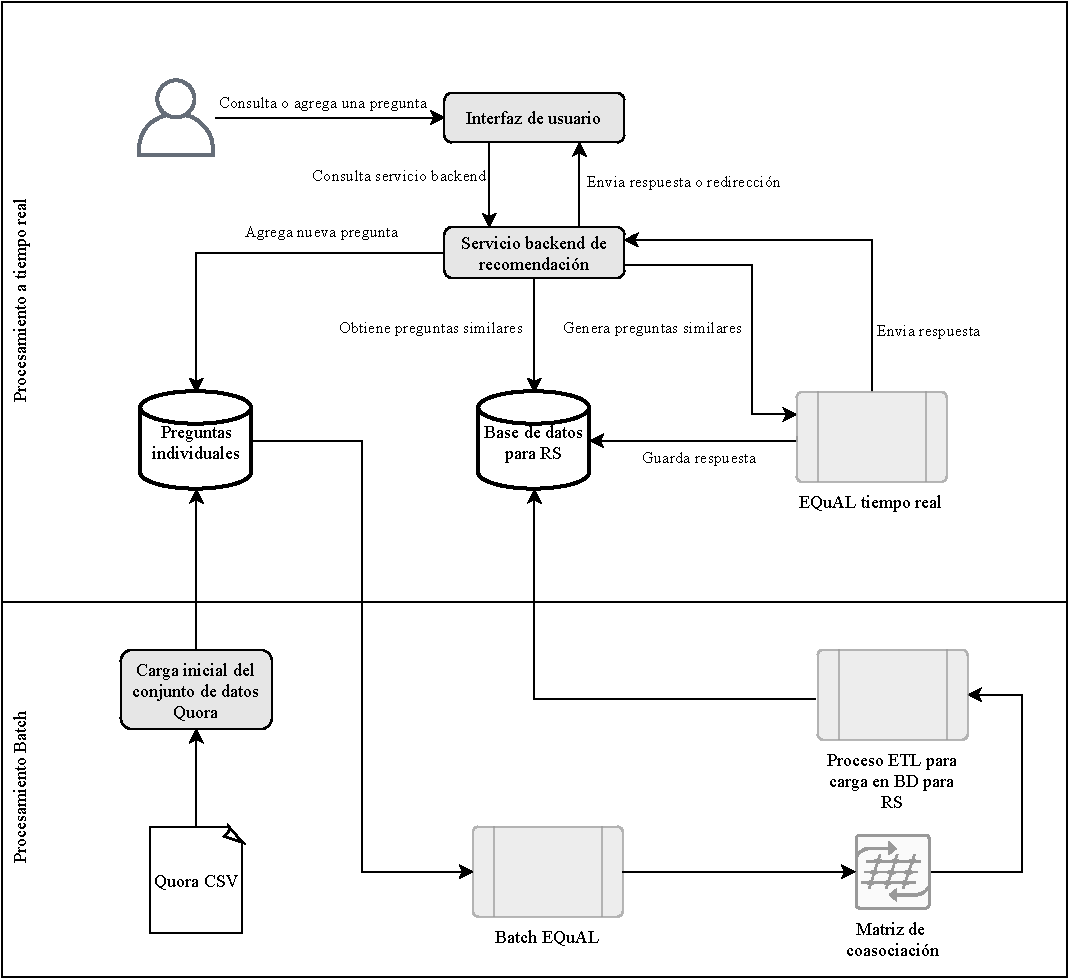
\includegraphics[width=0.9\linewidth]{8_problema_investigacion/imagenes/implementacion_rs}
	\caption{Arquitectura de un Sistema de Recomendación a tiempo real utilizando el método EQuAL.}
	\label{fig:implementacionrs}
\end{figure}

\subsubsection{Arquitectura general}
La arquitectura del RS embebido en un sitio de CQA colaborativo, consiste básicamente en un microservicio dedicado a recomendación, un artefacto de software que realizará la función de recomendación a tiempo real de forma distribuida, una base de datos altamente escalable NoSQL, y un proceso fuera de línea que generará una actualización de la misma de forma periódica.

\bigskip La Figura \ref{fig:implementacionrs} muestra cómo interactúa la totalidad de componentes relativos al RS, divididos fundamentalmente en procesamiento a tiempo real y fuera de línea; y además, muestra todas las interacciones posibles entre los componentes. En los siguientes apartados, se explicará cada uno de los tres casos de uso dentro de este sistema.

\subsubsection{Procesamiento fuera de línea}
La Figura \ref{fig:implementacionrsbatch} muestra el procesamiento fuera de línea para actualización y carga inicial de la base de datos que contendrá la matriz de co-asociación en un formato adecuado para consulta. Este proceso se ejecutará periódicamente, teniendo como entrada al conjunto de datos (en este ejemplo, el de Quora) en una base de datos. Para nuestro caso, esta base de datos sería inicializada con el conjunto de datos utilizado en este trabajo de tesis en forma de archivos de texto. A continuación se detallará cada uno de los casos.

\bigskip
\begin{figure}[h!]
	\centering
	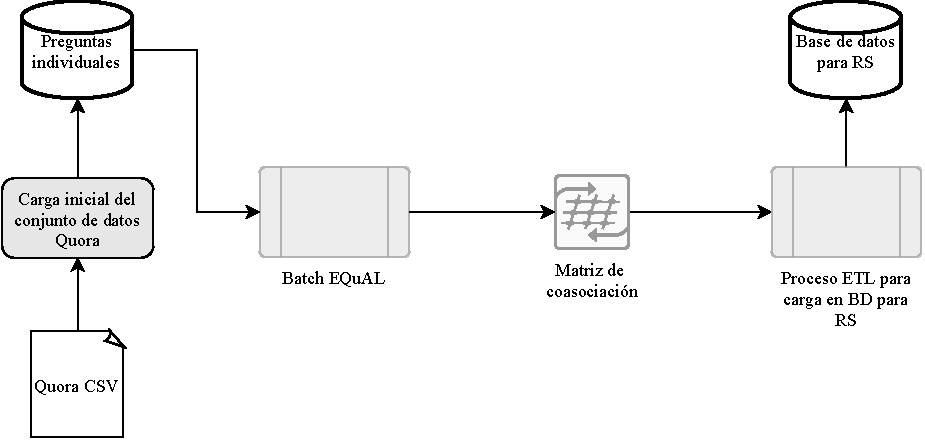
\includegraphics[width=0.9\linewidth]{8_problema_investigacion/imagenes/implementacion_rs_batch}
	\caption{Arquitectura de un sistema de recomendación a tiempo real utilizando el método EQuAL.}
	\label{fig:implementacionrsbatch}
\end{figure}

Como punto de partida, se carga inicialmente una base de datos con el conjunto de datos Quora original. Esta base de datos podría ser relacional, o de otro tipo, pero debería tener dos características principales: rápida inserción de registros y debe permitir obtener todos los registros de una tabla mediante una sola consulta. La inserción rápida es importante en el caso del agregado de una nueva pregunta en tiempo real. Por otro lado, la capacidad de seleccionar todos los registros de una tabla tiene importancia para el proceso fuera de línea que utilizará el método EQuAL para la actualización periódica del RS.

\bigskip De forma periódica, el proceso fuera de línea (en el cual se basa este trabajo) obtendrá todas las preguntas de la base de datos de preguntas individuales para crear la matriz de co-asociación. La periodicidad podrá variar dependiendo de la configuración y la arquitectura en la cual se ejecuta. Mientras más rápido sea este proceso, podría ser programado con más frecuencia. Podría ejecutarse, por ejemplo, diariamente, en momentos de bajo tráfico en el sitio en cuestión. Por otro lado, este proceso será el encargado de entrenar, de forma ad-hoc, los modelos que así lo requieran, y generar nuevos corpus que se nutrirán de nuevas palabras provenientes de preguntas nuevas agregadas por los usuarios una vez que el sistema esté en funcionamiento.

\bigskip
\begin{table}[h!]
	\footnotesize
	\caption{Matriz de co-asociación salida del proceso EQuAL.}
	\begin{tabularx}{\textwidth}{*{7}{>{\centering\arraybackslash}X}}
		\toprule
		\textbf{question\_id\_1} & \textbf{question\_id\_2} & \textbf{question\_1} & \textbf{question\_2} & \textbf{similarity} \\
		\midrule
		1 & 2 & question\_desc\_1 & question\_desc\_2 & 0.34 \\
		1 & 3 & question\_desc\_1 & question\_desc\_3 & 0.67 \\
		1 & 4 & question\_desc\_1 & question\_desc\_4 & 0.92 \\
		\bottomrule
	\end{tabularx}
	\label{tab:table-co-asociation}
\end{table}

Adicionalmente, un proceso ETL\footnote{Siglas para Extract, Transform and Load «extraer, transformar y cargar».}, que tendrá como origen la matriz de co-asociación, cargará la base de datos que guardará la información de similaridad entre preguntas y es consultada por el servicio de recomendación. Las características que debe tener esta base de datos serán descritas en el apartado siguiente. El proceso ETL podrá ser lanzado mediante un evento que indique que la nueva matriz de co-asociación ha sido generada, o bien podría ser una extensión del proceso EQuAL. Un ejemplo de la entrada de este procesamiento puede ser el que se muestra en la Tabla \ref{tab:table-co-asociation}, el cual muestra la matriz de co-asociación: las columnas \(question\_id\_1\) y \(question\_id\_2\) corresponden a los identificadores de preguntas, las columnas \(question\_1\) y \(question\_2\) corresponden al contenido de cada una de las preguntas, y la columna \(similarity\) indica cual es la similaridad entre las dos preguntas de cada una de las filas. Por ejemplo, la primera fila indica una similaridad de \(0.34\) entre las preguntas 1 y 2. Luego del proceso ETL, los registros de la base de datos para el RS tendrán la estructura que se muestra en la Tabla \ref{tab:table-similar-questions}, que posee solo tres columnas, el ID de pregunta (\(question\_id\)), su descripción (\(question\)), y la preguntas similares con su similaridad. Cada una de las preguntas similares está compuesta por un ID, la descripción y la similaridad con la pregunta correspondiente a la fila en cuestión (\(similar\_questions\)). Esto permitirá consultar la pregunta mediante su ID de manera muy eficiente. Por otro lado, la carga de la tabla también será muy eficiente, ya que la cantidad de registros se reduce a la cantidad de preguntas individuales, en lugar de la cantidad de registros de la matriz de co-asociación. La columna “similar\_questions” será en formato JSON, lo cual permite acceder a datos con una estructura definida, y serializar y deserializar los mismos de una forma estándar.

\bigskip Además, este proceso ETL podría ser utilizado para la actualización de índices o matrices en memoria utilizadas para un RS a tiempo real.

\begin{table}[h!]
	\centering
	\footnotesize
	\caption{Ejemplo de un registro de la base de datos de similaridad entre preguntas.}
	\begin{tabular}{|c|c|l|}
		\hline
		\textbf{question\_id} &
		\textbf{question} &
		\multicolumn{1}{c|}{\textbf{similar\_questions}} \\ \hline
		1 & question\_desc\_1 & \begin{lstlisting}[language=json]
[
	{
		"id": 4,
		"question": "question_desc_4",
		"similarity": "0.92"
	},
	{
		"id": 3,
		"question": "question_desc_3",
		"similarity": "0.67"
	},
	{
		"id": 2,
		"question": "question_desc_2",
		"similarity": "0.34"
	}
]
		\end{lstlisting} \\ \hline
	\end{tabular}
	\label{tab:table-similar-questions}
\end{table}

\subsubsection{Consulta de una pregunta existente}
En este apartado, se supone que la base de datos posee toda la información necesaria y está disponible; y además, que existe una aplicación web que consulta un servicio backend dedicado al Sistema de Recomendación, mediante una API REST\footnote{Representational State Transfer. Es una arquitectura y conjuntos de convenciones basada en servicios web para intercambios de información.}. Este último consultará la base de datos para devolver las preguntas similares a un ID de pregunta dado.

\begin{figure}[h!]
	\centering
	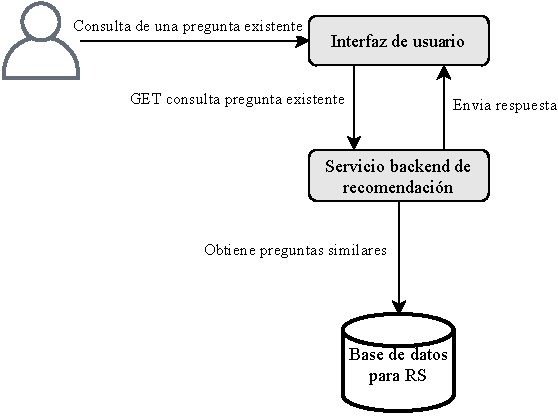
\includegraphics[width=0.6\linewidth]{8_problema_investigacion/imagenes/implementacion_rs_consulta}
	\caption{Flujo de consulta de una pregunta existente.}
	\label{fig:implementacionrsconsulta}
\end{figure}

La Figura \ref{fig:implementacionrsconsulta} muestra el flujo de la consulta de una pregunta existente. En el momento que un usuario consulta una pregunta en el sitio, el servicio frontend enviará una solicitud GET al servicio backend, utilizando el ID de la pregunta en cuestión. El servicio backend buscará la pregunta en la base de datos utilizando el ID de pregunta y retornando todas las preguntas similares. Las preguntas similares correspondientes pueden estar ordenadas por el valor de similaridad en forma decreciente. Esta operación debería ser ejecutada de manera rápida y eficiente, debido a que el servicio backend es dedicado al RS y la base de datos posee las siguientes características:
\begin{itemize}
	\item La información de similaridad entre preguntas estará almacenada en una tabla con una clave primaria simple (PK), formada solo por el ID de pregunta. Esta estructura genera un índice por ID de pregunta, lo cual posibilita una búsqueda rápida.
	\item La Tabla \ref{tab:table-similar-questions} podría estar particionada por la PK. Esto significa que se generan particiones de datos a lo largo de los diferentes nodos en el esquema de base de datos, basado en una función hash consistente y generada por el ID de pregunta. Esto es especial para búsquedas rápidas por PK, y además, facilita la escalabilidad horizontal y replicación.
	\item La información de preguntas similares para un ID dado, estará en formato JSON, haciendo que el servicio backend tenga un trabajo casi nulo para disponibilizar las preguntas similares al usuario final.
	\item Se recomienda una base de datos NoSQL ya que ellas vienen con un número de buenas prácticas arquitectónicas que afectan el rendimiento, tales como distribución de datos automática, baja latencia, consultas asíncronas, replicación de datos y alta disponibilidad.
\end{itemize}

\subsubsection{Agregar una nueva pregunta}\label{sec:implementacion_rs_agregar}
Esta funcionalidad es opcional y depende de los requerimientos del sitio y las funciones de recomendación a desarrollar, ya que recomendar ítems instantáneamente para un ítem recién agregado a un RS es un gran desafío para los arquitectos de software. Cabe aclarar que esta funcionalidad es opcional ya que, si los requerimientos del sistema no necesitan de la misma, se podría esperar a la ejecución del proceso fuera de línea, de tal forma que este asigne preguntas similares a la pregunta recién agregada. El propósito principal es realizar el cálculo en tiempo real de los ítems recomendados para el ítem recién agregado al sistema, hacerlos disponibles al usuario final, y que esto no signifique una sobrecarga del mismo. La recomendación en tiempo real será provisoria hasta que esta pregunta sea tenida en cuenta por el proceso fuera de línea y se encuentre disponible en la base de datos del RS, por lo cual esta funcionalidad puede ser utilizada como respaldo en el caso de que una pregunta no sea encontrada en dicha base de datos. La arquitectura propuesta a continuación, que se detalla en la Figura \ref{fig:implementacionrsagregar}, propone el cálculo de similaridad a tiempo real, utilizando métodos derivados del método EQuAL que sean apropiados y tengan buen desempeño. Esto permitirá que no solamente los usuarios del sitio puedan tener acceso a las preguntas de manera inmediata, sino que estas también sean accesibles al mismo usuario que agregó la pregunta, evitando así, el tiempo de espera para que su pregunta sea respondida.

\begin{figure}[h!]
	\centering
	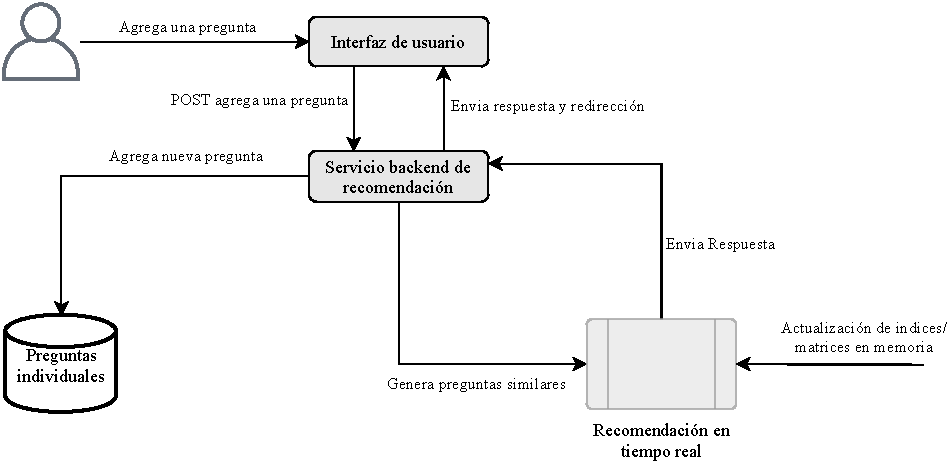
\includegraphics[width=0.9\linewidth]{8_problema_investigacion/imagenes/implementacion_rs_agregar}
	\caption{Flujo en el RS a tiempo real cuando se agrega una nueva pregunta al sistema.}
	\label{fig:implementacionrsagregar}
\end{figure}

\bigskip Cuando se agrega una nueva pregunta, la información es enviada al servicio backend mediante una solicitud POST, el cual es enviado al módulo que realiza el cálculo de recomendación a tiempo real. Este último retorna las preguntas similares para que estén disponibles al usuario. Luego de efectuar la pregunta, el usuario puede ser redireccionado a una URL que contenga la pregunta recién agregada y las preguntas similares. Por otro lado, y de manera asíncrona, el servicio backend guarda la pregunta recién agregada a la base de datos de preguntas individuales, para que sea tenida en cuenta en la próxima ejecución del proceso fuera de línea.

\bigskip El módulo de recomendación en tiempo real podría realizar el cálculo de recomendación con distintos enfoques. A continuación, se mencionan propuestas, que quedan fuera del alcance de esta tesis, para implementar arquitecturas de buen desempeño utilizando enfoque de Big Data.

\subparagraph{Cálculo de similaridad contra todas las preguntas del sitio}
En este enfoque, de ser posible, este módulo debería mantener la matriz de co-asociación en memoria, para poder realizar el cálculo a demanda. La pregunta recién ingresada debe compararse con todas las preguntas del sitio. Al mismo tiempo, se quiere tener control del tamaño de la matriz. Para tal fin, es posible mantener solo una fracción de la misma con los datos más importantes. Existen diversas técnicas para llevarlo a cabo, por ejemplo implementar un algoritmo de \textit{Caché de Reemplazo Adaptativo }(ARC\footnote{Por sus siglas en inglés \textit{Adaptive Replacement Cache}.}) que descarta los objetos que no fueron usados recientemente y los objetos con menor frecuencia de uso. Por otro lado, las preguntas, como se describió anteriormente, deben tener un identificador único. Por lo cual, cada registro en el caché puede ser asignado a una pregunta. Con identificadores en el rango \(0.. N-1\) si \(N\) es la cantidad total de registros en el caché.

\bigskip En cuanto al cálculo de similaridad, los modelos que lo requieran deben estar pre-entrenados y cargados en memoria. Por ejemplo, podría ser posible que una nueva pregunta realice una comparación con todas las preguntas en caché (fuerza bruta) utilizando cada uno de los algoritmos de similaridad. El proceso de ensamble de clustering puede ser simplificado a la media de los valores calculados por los algoritmos de similaridad subyacentes, para luego retornar las k preguntas más similares a la recién agregada.

\subparagraph{Búsqueda de vecinos cercanos con representaciones vectoriales}
Este enfoque utiliza representaciones vectoriales de cada una de las preguntas individuales. Para tal fin, es posible que el método EQuAL que se ejecuta periódicamente genere una representación vectorial de cada una de las preguntas, utilizando uno de los métodos (o varios de ellos combinados) que usan este tipo de representación como paso intermedio del cálculo de similaridad. Con este listado de preguntas en forma de vector, es posible cargar un índice en memoria que permita la búsqueda de un conjunto de vectores inmediatamente.

\bigskip Mediante una nueva pregunta agregada al sistema y su representación vectorial, es posible buscar sus \(k\) vecinos más cercanos. Este método de clasificación es llamado \textit{KNN} (del inglés \textit{k-Nearest-Neighbors}). Para un registro \(t\) a ser clasificado, sus \(k\) vecinos más cercanos son obtenidos en la forma de vecinos de \(t\) \citep{guo2003knn}. Este método es utilizado por varias librerías reconocidas por la industria, tales como Annoy \footnote{Spotify Annoy GitHub Repository: \url{https://github.com/spotify/annoy}. Último acceso: Junio 2021.}, las cuales poseen un muy buen desempeño y realizan un uso muy eficiente de memoria.

\subparagraph{Modelos de scoring}
Es posible utilizar el proceso ETL como parte del procesamiento fuera de línea para cargar un motor de búsqueda que contenga índices basados en scoring. Ciertas herramientas, tales como ElasticSearch\footnote{Sitio web ElasticSearch: \url{https://www.elastic.co/}. Último acceso: Junio 2021.}, tienen la capacidad de devolver documentos similares a uno consultado basándose en la generación de índices. El listado de preguntas puede ser tomado como entrada para la generación del mismo. Cada uno de los documentos es indexado. Los términos presentes en cada una de las preguntas (documentos) son descompuestos e indexados de forma invertida. Cada término es indexado, y contendrá, por ejemplo, en qué posición dentro de cada documento se encuentra. En el momento de una nueva consulta, se devuelven todos los documentos que coinciden con la misma. Con el fin de dar relevancia a los mismos, cada uno de los documentos tiene asignado un score que es calculado con el método TF-IDF (tal como se explicó anteriormente), es decir que un término que se encuentra varias veces en el documento consultado pero es contenido por pocos documentos en el índice, tendrá más relevancia que un término que aparece con más frecuencia en distintos documentos. Entonces, la relevancia de cada uno de los documentos retornados, depende (en parte) del peso de cada término en el documento consultado.

\subsubsection{Condiciones institucionales para el desarrollo de la tesis. Infraestructura y equipamiento}
El presente trabajo se lleva a cabo en el marco del Proyecto PID UTN: Minería de Datos aplicado a problemáticas de Big Data de la Universidad Tecnológica Nacional, Facultad Regional Rosario\footnote{Código del PID: SIUTNRO0005006. Bajo la dirección del Ing. Eduardo Amar.}.

\bigskip El tesista cursó la Maestría en Ingeniería en Sistemas de Información en dicha Facultad y contó con el equipamiento e instalaciones del Departamento en Ingeniería en Sistemas de Información. Con el objetivo de realizar el desarrollo tecnológico de este trabajo de tesis, el tesista utilizó equipos propios así como también los equipos de la universidad, cuando fue necesario. Los conjuntos de datos para la experimentación y validación de la solución propuesta están disponibles libremente en Internet, así como también el software y herramientas necesarias.

















